\noindent

\includegraphics[height=1.25cm]{images/pictograms/benchmark}

\includegraphics[height=1.25cm]{images/pictograms/FEM}

\includegraphics[height=1.25cm]{images/pictograms/wave}

%%%%%%%%%%%%%%%%%%%%%%%%%%%%%%%%%%%%%%%%%%%%%%%%%%%%%%%%%%%%%%%%%%%%%%%%%%%%%%%%%%%%%%%%%%%%%%%%%%%

\begin{flushright} {\tiny {\color{gray} python\_codes/fieldstone\_164/text.tex}} \end{flushright}

%\lstinputlisting[language=bash,basicstyle=\small]{python_codes/template_keywords.key}

\par\noindent\rule{\textwidth}{0.4pt}

\begin{center}
\inpython
{\small Code: \url{https://github.com/cedrict/fieldstone/tree/master/python_codes/fieldstone_164}}
\end{center}

\par\noindent\rule{\textwidth}{0.4pt}

%%%%%%%%%%%%%%%%%%%%%%%%%%%%%%%%%%%%%%%%%%%%%%%%%%%%%%%%%%%%%%%%%%%%%%%%%%%%%%%%%%%%%%%%%%%%%%%%%%%

This \stone solves the 1d wave equation using 1st order finite elements. 
The theory is presented in Chapter~\ref{MMM-fem_waveq}. 


The mesh is built simply
\begin{lstlisting}
x=np.linspace(0,Lx,nnx)
\end{lstlisting}
The connectivity array is also very simple in 1d:
\begin{lstlisting}
icon=np.zeros((m,nelx),dtype=np.int32)
for iel in range(0,nelx):
    icon[0,iel]=iel
    icon[1,iel]=iel+1
\end{lstlisting}
where $m$ is the number of nodes per element and $nelx$ the number of elements.

Depending on the method we will need some or all of these arrays:
$\vec{\cal U}(t)$ (\lstinline|uprev| array), 
$\vec{\cal U}(t-dt)$ (\lstinline|uprevprev| array), 
$\vec{\cal U}(t+dt)$ (\lstinline|u| array), 
$\vec{\dot{{\cal U}}}(t)$ (\lstinline|udotprev| array), 
$\vec{\dot{{\cal U}}}(t+dt)$ (\lstinline|udot| array).
All these are $nnx=nelx+1$ long. 
In the code we declare and initialise them as follows 
\begin{lstlisting}
u=np.zeros(nnx,dtype=np.float64)    
uprevprev=np.zeros(nnx,dtype=np.float64) 
uprev=np.zeros(nnx,dtype=np.float64)     
udot=np.zeros(nnx,dtype=np.float64)      
udotprev=np.zeros(nnx,dtype=np.float64) 
if method==1 or method==2:
   t=2*dt
   for i in range(0,nnx):
       uprevprev[i]=u_th(x[i],0)
       uprev[i]=u_th(x[i],0)+dt*udot_th(x[i],0)
if method==3:
   t=dt
   for i in range(0,nnx):
       uprev[i]=u_th(x[i],0)
       udotprev[i]=udot_th(x[i],0)
\end{lstlisting}

Note that methods 1 and 2 require two previous solutions to start, so
the first solution we obtain is at time $t=2\; dt$, while method 3
only needs one previous solution so it starts at time $t=dt$.

This code implements all three methods dealing with the second-order time derivative. 
I recall these here briefly hereafter.
%We start from the following equation
%\[
%\M \cdot \vec{\ddot{{\cal U}}}(t) + c^2 \K \cdot \vec{\cal U}(t) = \vec{0}
%\]

\begin{itemize}
%................................
\item method \# 1a
\[
\M \cdot  \vec{\cal U}(t+dt)
= [2  \M  - c^2 dt^2 \K  ]  \cdot \vec{\cal U}(t) - \M \cdot \vec{\cal U}(t-dt)
\]

The code structure is then as follows:
\begin{lstlisting}
for istep in range(0,nstep):
    for iel in range(0,nelx):
        for k in range(0,m):
            up[k]=uprev[icon[k,iel]]
            upp[k]=uprevprev[icon[k,iel]]
        a_el[:,:]=Me[:,:]
        b_el[:]=(2*Me-c**2*dt**2*Ke).dot(up)-Me.dot(upp)
        #apply b.c.
        #assemble
    # end for
    u=sps.linalg.spsolve(sps.csr_matrix(A_mat),rhs)
    ...
    ...
    uprevprev[:]=uprev[:]
    uprev[:]=u[:]
# end for
\end{lstlisting}

%................................
\item method \# 1b
\[
(\M + c^2 \delta t^2 \K ) \cdot \vec{\cal U}(t+\delta t) 
= \underbrace{ \M \cdot(2 \vec{\cal U}(t) - \vec{\cal U}(t-\delta t)) }_{\vec{b}}
\] 

The code structure is then as follows:
\begin{lstlisting}
for istep in range(0,nstep):
    for iel in range(0,nelx):
        for k in range(0,m):
            up[k]=uprev[icon[k,iel]]
            upp[k]=uprevprev[icon[k,iel]]
        a_el[:,:]=Me[:,:]+c**2*dt**2*Ke
        b_el[:]=Me.dot(2*up-upp)
        #apply b.c.
        #assemble
    # end for
    u=sps.linalg.spsolve(sps.csr_matrix(A_mat),rhs)
    ...
    ...
    uprevprev[:]=uprev[:]
    uprev[:]=u[:]
# end for
\end{lstlisting}

%................................
\item method \# 2 
\[
\M \cdot \vec{\cal W}= -c^2 \K \cdot \vec{\cal U}(t)
\]
\[
\vec{\cal U}(t+dt) = dt^2 \; \vec{\cal W} +2 \vec{\cal U}(t) - \vec{\cal U}(t-dt)
\]
\begin{lstlisting}
for istep in range(0,nstep):
    for iel in range(0,nelx):
        for k in range(0,m):
            up[k]=uprev[icon[k,iel]]
        a_el[:,:]=Me[:,:]
        b_el=-c**2*Ke.dot(up)
        #apply b.c.
        #assemble
    # end for
    uu=sps.linalg.spsolve(sps.csr_matrix(A_mat),rhs)
    u=np.zeros(nnx,dtype=np.float64)  
    u[:]=dt**2*uu[:]+2*uprev[:]-uprevprev[:]
    ...
    ...
    uprevprev[:]=uprev[:]
    uprev[:]=u[:]
# end for
\end{lstlisting}

%................................
\item method \# 3

\begin{align}
\vec{\cal U}(t+dt) = \vec{\cal U}(t) + dt \; \vec{\dot{{\cal U}}}(t) \\
\M \cdot \frac{\vec{\dot{{\cal U}}}(t+dt)-\vec{\dot{{\cal U}}}(t) }{dt}  &= -c^2 \K \cdot \vec{\cal U}(t) 
\end{align}
\begin{lstlisting}
for istep in range(0,nstep):
    for iel in range(0,nelx):
        for k in range(0,m):
            up[k]=uprev[icon[k,iel]]
        a_el[:,:]=Me[:,:]
        b_el=-c**2*Ke.dot(up)
        #apply b.c.
        #assemble
    # end for
    u[:]=uprev[:]+udotprev[:]*dt
    R=sps.linalg.spsolve(sps.csr_matrix(A_mat),rhs)
    udot[:]=udotprev[:]+dt*R[:]
    ...
    ...
    uprev[:]=u[:]
    udotprev[:]=udot[:]
# end for
\end{lstlisting}





 
\end{itemize}
At this stage we notice that the FE matrix is simply the 
mass matrix for all three methods (unless the implicit
variant of method 1 is used). 



As shown in Section XXX the mass matrix $\M$ and Laplace matrix $\K$ are 
easily analytically computed for linear 1D elements:
\[
\M_e=
h_x\frac{1}{3}
\left(
\begin{array}{cc}
1 & 1/2 \\ 1/2 & 1
\end{array}
\right)
=
\left(
\begin{array}{cc}
h_x/3 & h_x/6 \\ h_x/6 & h_x/3
\end{array}
\right)
\qquad
\K_e=
\frac{1}{h_x}
\left(
\begin{array}{cc}
1 & -1 \\ -1 & 1
\end{array}
\right)
\]
This translates as follows in the code:
\begin{lstlisting}
Me=np.array([[hx/3,hx/6],[hx/6,hx/3]],dtype=np.float64)
Ke=np.array([[1/hx,-1/hx],[-1/hx,1/hx]],dtype=np.float64)
\end{lstlisting}

Let us consider a test case with three elements. 
The first elemental matrix $\M_e$
gets modify by the application of the boundary conditions:
\begin{verbatim}
[[0.11111111 0.        ]
 [0.         0.11111111]]
\end{verbatim}
The second elemental matrix is simply $\M_e$
\begin{verbatim}
[[0.11111111 0.05555556]
 [0.05555556 0.11111111]]
\end{verbatim}
and the third elemental matrix is also modified bc of boundary conditions:
\begin{verbatim}
[[0.11111111 0.        ]
 [0.         0.11111111]]
\end{verbatim}
When assembled we obtain the following FE matrix:
\begin{verbatim}
[[0.11111111 0.         0.         0.        ]
 [0.         0.22222222 0.05555556 0.        ]
 [0.         0.05555556 0.22222222 0.        ]
 [0.         0.         0.         0.11111111]]
\end{verbatim}

The code consists of a time loop, and inside each iteration 
the FE matrix and rhs are re-built (technically the FE matrix 
is the same every time), the system solved, and the solution
exported to an ascii file for later processing.

%==============================================================================
\section*{Results - Experiment \# 1}

The problem at hand is described in Section~\ref{MMM-ss:sw1d}.
As such we first create two functions:

\begin{lstlisting}
def u_th(x,t):
    return np.cos(2*np.pi*t)*np.sin(2*np.pi*x)

def udot_th(x,t):
    return -2*np.pi*np.sin(2*np.pi*t)*np.sin(2*np.pi*x)
\end{lstlisting}

The total energy is then
\begin{eqnarray}
\left\|  \frac{\partial u}{\partial t} (\cdot, t)  \right\|^2 + 
c^2 \left\|  \frac{\partial u}{\partial x} (\cdot, t)  \right\|^2
&=&
\left\|  -2\pi \sin(2 \pi t) \sin (2 \pi x)  \right\|^2 + 
c^2 \left\|  -2\pi \cos (2\pi t) \sin(2 \pi x)  \right\|^2 \nn\\
&=&
\int_0^1 \left(  -2\pi \sin(2 \pi t) \sin(2 \pi x) \right)^2 dx
+\int_0^1 \left(  -2\pi \cos (2\pi t) \sin(2 \pi x) \right)^2 dx \nn\\
&=&
4\pi^2 \sin^2(2 \pi t) \int_0^1  \sin^2(2 \pi x)  dx
+4\pi^2 \cos^2(2 \pi t)\int_0^1  \cos^2(2 \pi x)  dx \nn\\
&=&  4\pi^2 \sin^2(2 \pi t) \frac12 +  4\pi^2 \cos^2(2 \pi t) \frac12  \nn\\
&=&  2\pi^2 (\sin^2(2 \pi t) + \cos^2(2 \pi t) )   \nn\\
&=& 2 \pi^2 \nn\\
&\simeq& 19.7392
\end{eqnarray}


The time step is set to $dt=10^{-3}$. 
The following results are obtained for $nelx=20$ with all three methods.

\begin{center}
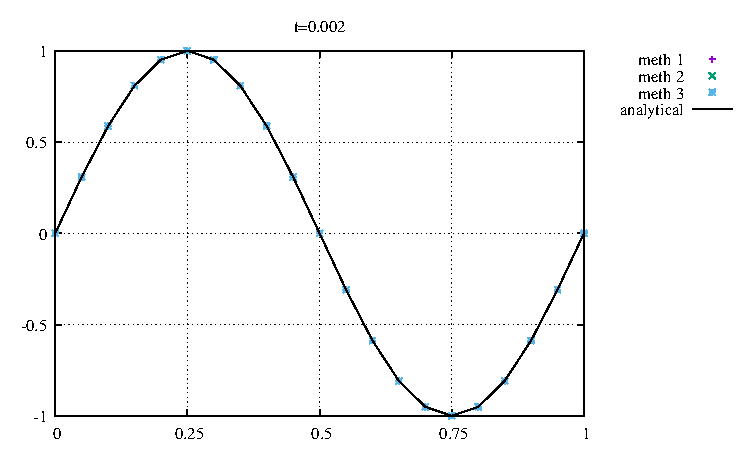
\includegraphics[width=8cm]{python_codes/fieldstone_164/results1/u_0.pdf}
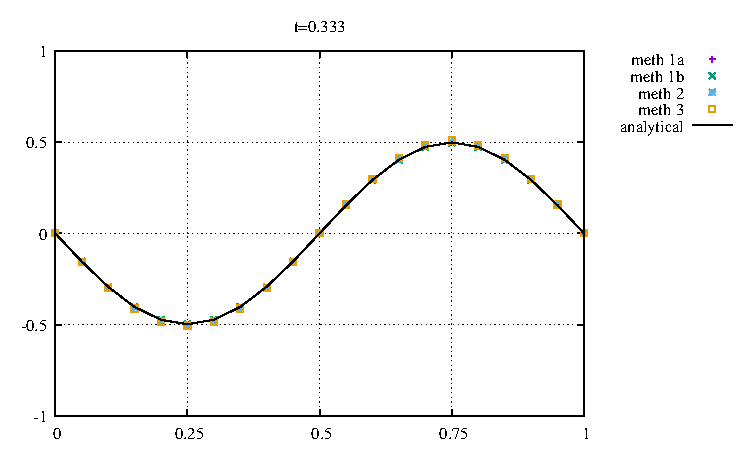
\includegraphics[width=8cm]{python_codes/fieldstone_164/results1/u_1.pdf}\\
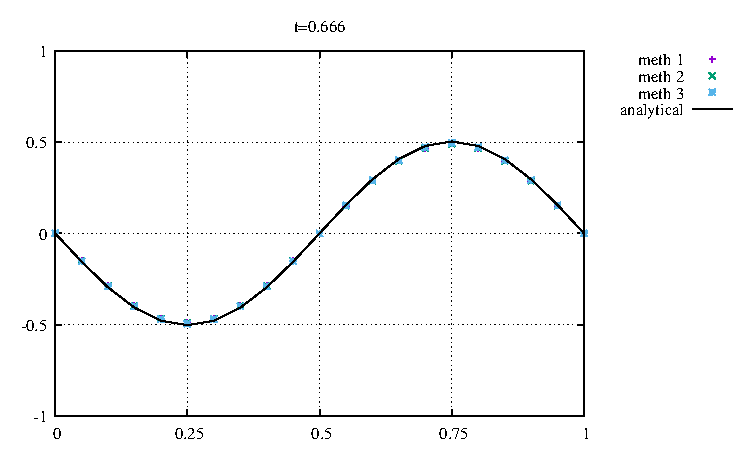
\includegraphics[width=8cm]{python_codes/fieldstone_164/results1/u_2.pdf}
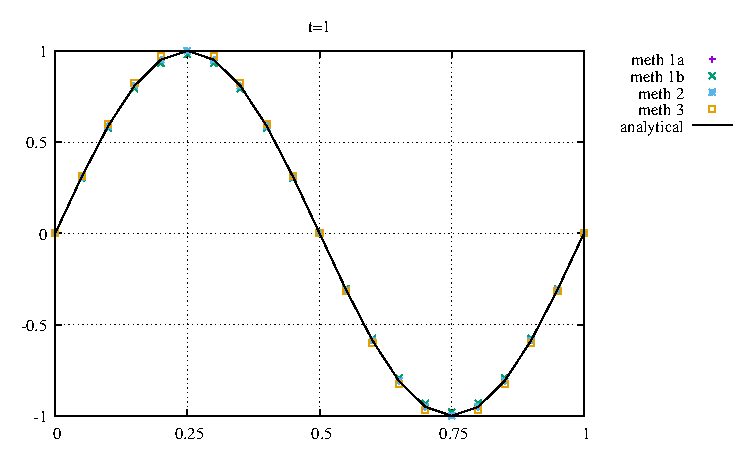
\includegraphics[width=8cm]{python_codes/fieldstone_164/results1/u_3.pdf}\\
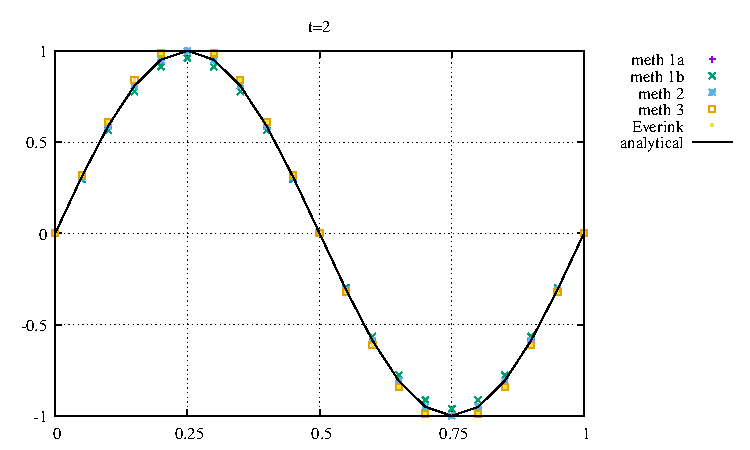
\includegraphics[width=8cm]{python_codes/fieldstone_164/results1/u_4.pdf}
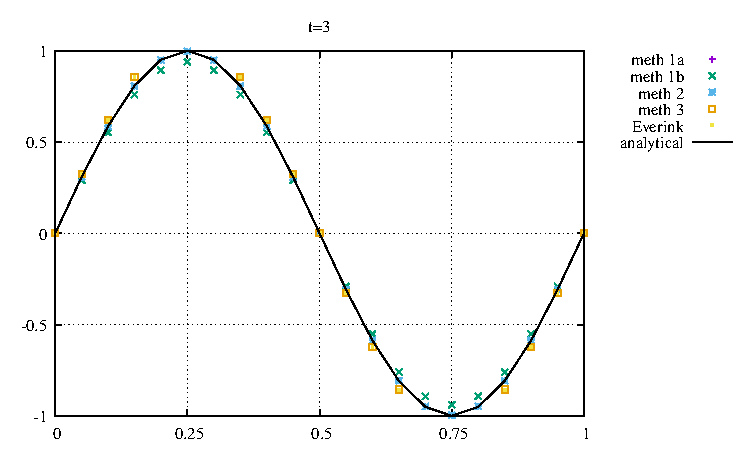
\includegraphics[width=8cm]{python_codes/fieldstone_164/results1/u_5.pdf}\\
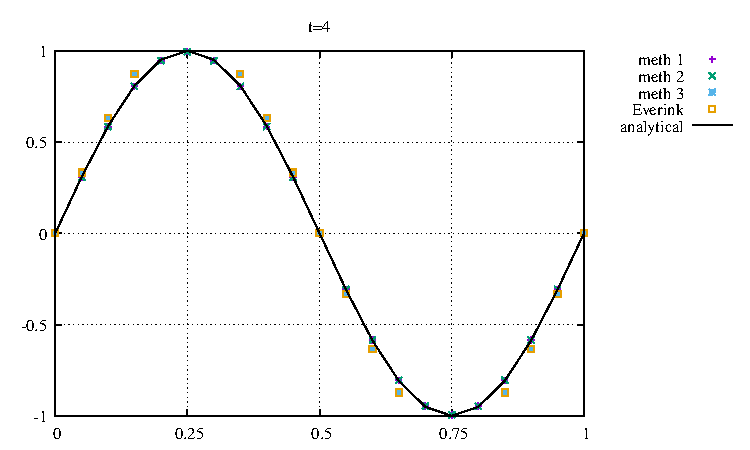
\includegraphics[width=8cm]{python_codes/fieldstone_164/results1/u_6.pdf}
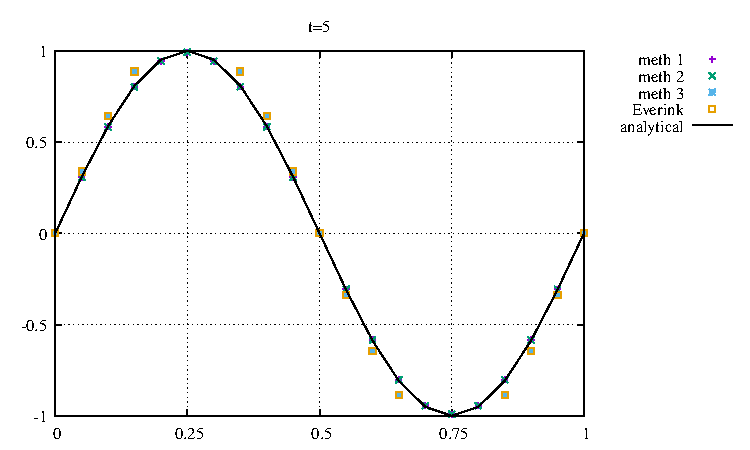
\includegraphics[width=8cm]{python_codes/fieldstone_164/results1/u_7.pdf}
\end{center}
We find that methods 1a and 2 seem to be more accurate than method 3.
To make sure I plot the results of Everink obtained with method 3 against mine 
and recover identical values.
Method 2b seems diffusive, i.e. min/max values decrease over time.

One can also look at the min/max values of $u$ for all three methods and 
for various resolutions:
\begin{center}
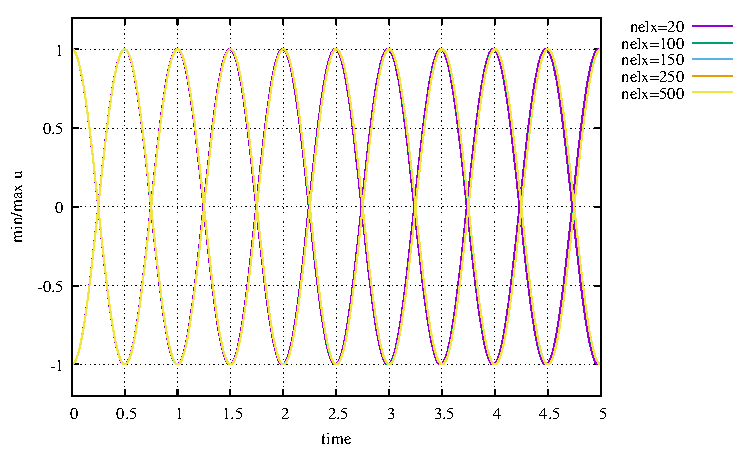
\includegraphics[width=7cm]{python_codes/fieldstone_164/results1/stats_meth1a.pdf}
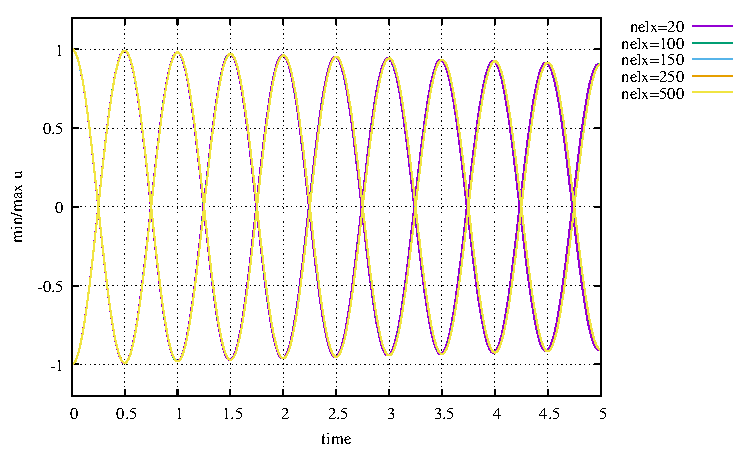
\includegraphics[width=7cm]{python_codes/fieldstone_164/results1/stats_meth1b.pdf}\\
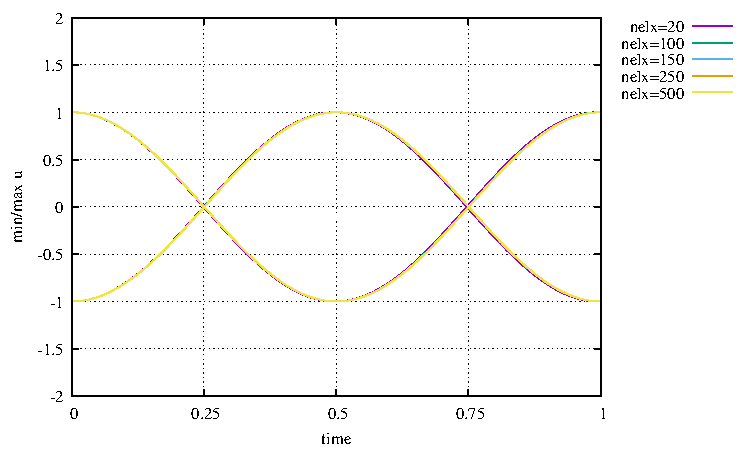
\includegraphics[width=7cm]{python_codes/fieldstone_164/results1/stats_meth2.pdf}
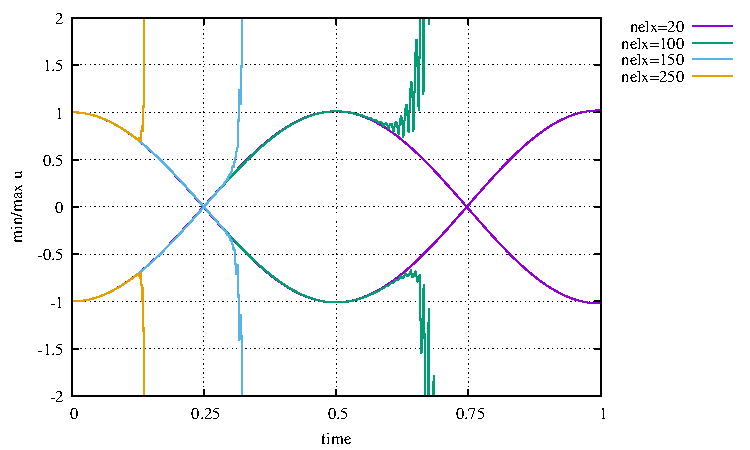
\includegraphics[width=7cm]{python_codes/fieldstone_164/results1/stats_meth3.pdf}
\end{center}
We find that method 3 is prone to numerical explosion, and method 
1b is prone to diffusion so they should probably be avoided.

Finally we can also monitor the total energy in the system over time, for all 
methods and for various resolutions:
\begin{center}
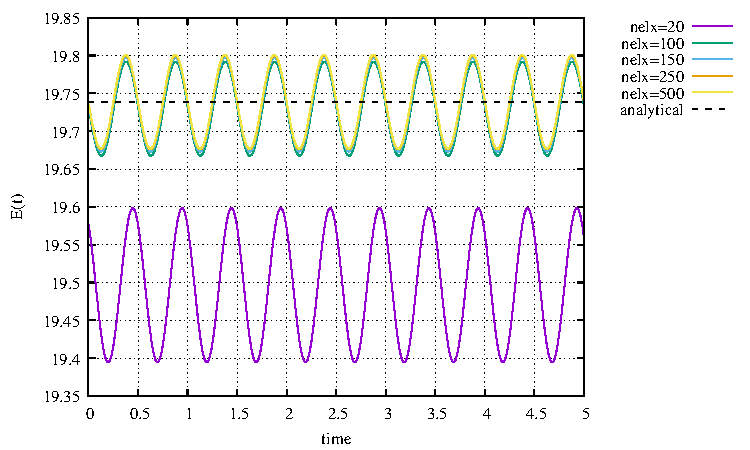
\includegraphics[width=7cm]{python_codes/fieldstone_164/results1/energy_meth1a.pdf}
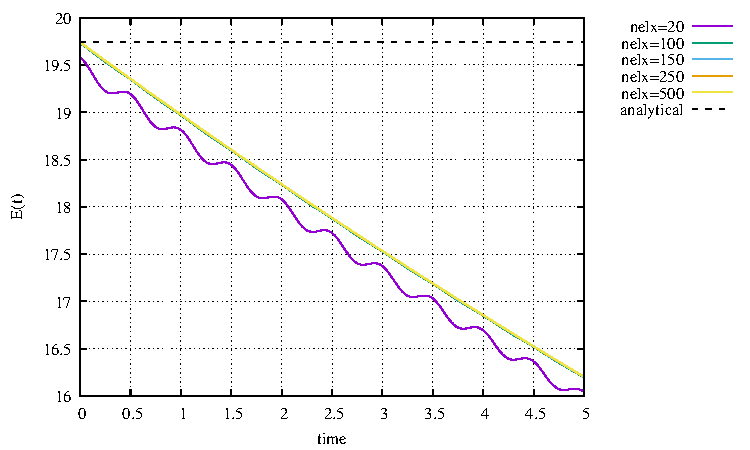
\includegraphics[width=7cm]{python_codes/fieldstone_164/results1/energy_meth1b.pdf}\\
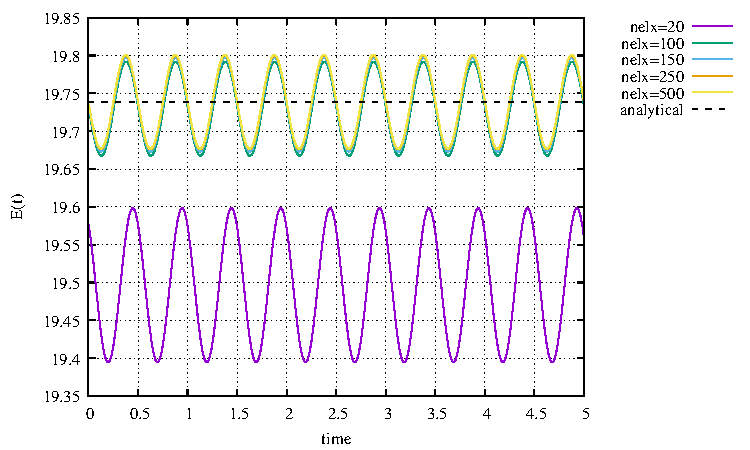
\includegraphics[width=7cm]{python_codes/fieldstone_164/results1/energy_meth2.pdf}
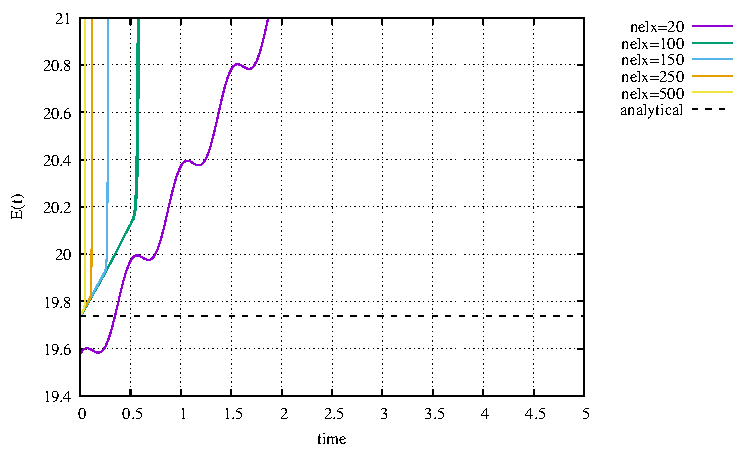
\includegraphics[width=7cm]{python_codes/fieldstone_164/results1/energy_meth3.pdf}
\end{center}

The conclusion is very clear. Again, only methods 1a and 2 seem to conserve
the total energy.

%==============================================================================
\section*{Results - Experiment \# 2}

In this case $L_x=1.5\pi\simeq 4.712$, $t_{final}=240$, 
\[
u(x,t=0)=2 \exp\left(-(x-L_x/2)^2 \right)+x/L_x
\qquad
\dot{u}(x,t=0)=0 
\]
Boundary conditions are given by $u(0)$ on the left and $u(L)$ on the right.
This experiment is borrowed from there\footnote{\url{https://juliateachingctu.github.io/Julia-for-Optimization-and-Learning/stable/lecture_13/ode/}}.

\begin{center}
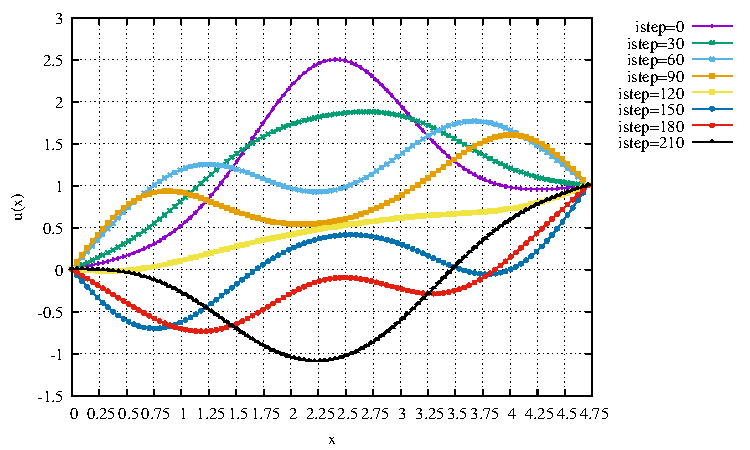
\includegraphics[width=12cm]{python_codes/fieldstone_164/results2/u.pdf}
\end{center}




